\documentclass[10pt,twocolumn]{article}
\usepackage[margin=1.5cm]{geometry}
\usepackage{times}
\usepackage{booktabs}
\usepackage{graphicx}
\usepackage{amsmath}
\usepackage{hyperref}
\usepackage{microtype}
\usepackage{parskip}
\setlength{\parskip}{3pt}
\setlength{\columnsep}{0.6cm}

\title{\textbf{Distribution-Matched Pair Classification\\for Cross-Geo Product Grouping}}
\author{NI-ADM 2026 -- GLAMI Product Matching Challenge}
\date{}

\begin{document}
\maketitle
\thispagestyle{empty}

%% ── 1. Introduction ──────────────────────────────────────────────────────────
\section{Introduction}

Cross-geo product matching requires identifying identical products spread
across listings from different countries, where titles may be in different
languages, images may differ in crop and background, and prices are expressed
in different currencies.
The GLAMI dataset~\cite{glami} contains approximately 1.3M fashion items from
multiple European markets, labelled with 217k distinct product identities.
The two competition tasks are (1) binary detection of duplicate-containing
groups (Phase~1) and (2) hard clustering of all items into product groups
(Phase~2), evaluated by pairwise F1.

The core difficulty is the gap between a retrieval model that must cover all
true matches and a precision-oriented classifier that must not merge distinct
products. Two additional challenges distinguish this dataset from standard
entity matching: (i)~the same product may have a Czech title in one listing
and a Romanian title in another, making lexical signals useless, and (ii)~the
inference candidate distribution is narrower than the training distribution,
causing naive classifiers to be miscalibrated.

Our system addresses both challenges: multimodal contrastive fine-tuning
provides language-agnostic embeddings, and a distribution-matched pair
classifier is trained on exactly the similarity range seen at inference.

%% ── 2. Related Work ─────────────────────────────────────────────────────────
\section{Related Work}

\paragraph{Zalando end-to-end product matching.}
The most directly related work is Tóth et al.~\cite{zalando}, who present an
industry-scale system for cross-geo duplicate detection in fashion e-commerce.
Their approach projects pretrained image and text encoders into a shared space
via contrastive learning and outperforms both single-modality systems and
large pretrained models such as CLIP. A human review loop is used in production
to achieve near-perfect precision.
Our work differs in two important respects.
First, we target a fully automated system without human review, which forces
the classifier to be more precise.
Second, and more fundamentally, we identify and correct the \emph{calibration
mismatch} that arises in the retrieve-then-rerank pipeline: Tóth et al.\ do
not discuss training the reranker on the same similarity region it will
encounter at inference, whereas we show this is the single most important
factor in our ablation (9-point F1 gap).

\paragraph{Entity matching with language models.}
DITTO~\cite{ditto} and DeepMatcher~\cite{deepmatcher} apply pre-trained
transformers to textual entity matching. They achieve strong results in
English, but neither addresses the cross-lingual or multimodal setting
required here.

\paragraph{Multimodal contrastive learning.}
CLIP~\cite{clip} demonstrated that joint image-text contrastive training
produces powerful shared representations. We extend this idea in a
supervised, domain-adapted setting: fine-tuning separate text and image towers
with ANCE hard-negative InfoNCE to align cross-geo product pairs in the GLAMI
fashion domain.

\paragraph{Approximate nearest-neighbour reranking.}
The two-stage retrieve-then-rerank paradigm (FAISS~\cite{faiss} +
classifier) is standard in dense retrieval. Our key contribution is
recognising that the \emph{reranker must be trained on the same similarity
distribution as the candidate set it will score}, not on the full pair
distribution.

%% ── 3. Methodology ──────────────────────────────────────────────────────────
\section{Methodology}

\begin{figure}[t]
  \centering
  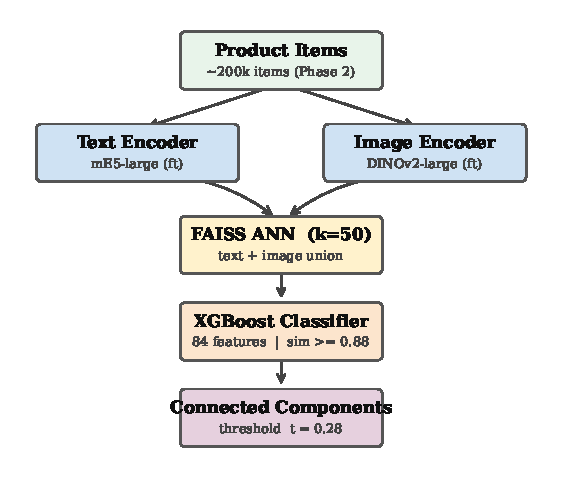
\includegraphics[width=\columnwidth]{fig_pipeline.pdf}
  \caption{System overview. Fine-tuned text and image encoders feed a FAISS
    union-of-neighbours retrieval stage; a distribution-matched XGBoost
    classifier scores each candidate pair; connected components produce the
    final product groups.}
  \label{fig:pipeline}
\end{figure}

\subsection{Multimodal Encoder Fine-tuning (ANCE)}

We fine-tune two separate 1024-dimensional backbone encoders using
Approximate Nearest-Neighbour Contrastive Estimation (ANCE):

\textbf{Text tower:} \texttt{intfloat/multilingual-e5-large}, avg-pooled
with the \texttt{query:} prefix.

\textbf{Image tower:} \texttt{facebook/dinov2-large}, CLS token.

Both towers are projected to 512~dimensions for contrastive training, but
the 1024-dimensional backbone output is used at inference.
Training proceeds in two phases: (1)~a warm-up phase with random in-batch
negatives (InfoNCE, temperature $\tau = 0.05$) to domain-adapt both
encoders to GLAMI fashion products, and (2)~a hard-negative refinement
phase where, per epoch, FAISS retrieves the nearest neighbours with a
\emph{different} label and inserts them explicitly into the InfoNCE
denominator. Models are trained sequentially to fit within 12 GB VRAM,
with gradient checkpointing enabled on both large backbones.

\subsection{Candidate Generation}

For each item we retrieve the top-50 text neighbours and top-50 image
neighbours separately using FAISS IVF (NLIST=500, NPROBE=25, inner
product metric). The two neighbour sets are unioned to form candidate
pairs. Using both modalities is critical: cross-geo pairs with different
language titles have low text similarity but moderate image similarity,
so a text-only index would miss them as candidates.

The combined similarity $s = 0.5 \cdot s_\text{text} + 0.5 \cdot s_\text{img}$ is
pre-computed for each candidate pair. All pairs with $s < 0.88$ are
discarded; the typical Phase~2 item has $\sim$20--60 surviving candidates.

\subsection{Distribution-Matched Pair Classifier}

Candidate pairs after FAISS filtering have $s \geq 0.88$ by construction.
A broadly-trained XGBoost classifier assigns near-$1.0$ probability to
every such pair because it has seen the full training distribution ($s$
ranging from $0$ to $1$), where $s \geq 0.88$ correlates almost perfectly
with same-label in the training data.

\textbf{Key insight}: we retrain the XGBoost classifier on
\emph{exactly the $s \geq 0.88$ region}, where both positives and
negatives are abundant (hard negatives share a brand, department, or
similar price but belong to different products). This distribution
shift makes the model learn the fine-grained discriminative features
that matter at inference.

\textbf{Features} (84 total): 20 base features including text cosine
similarity, image cosine similarity, L2 distances, element-wise
difference statistics (mean/std/max for both modalities), combined
similarity $s$, $|s_\text{text} - s_\text{img}|$, price ratio, price
difference, and exact-match indicators for department, colour, and brand;
plus 32 text PCA difference features and 32 image PCA difference features
(PCA fit on 50k training items, dim=32 each).

\textbf{Training}: 80k positives and 240k negatives mined from the
training set (all with $s \geq 0.88$), 1500-estimator XGBoost with
early stopping. Val AUC~=~0.9990, Val F1~=~0.9884 at $t=0.30$.

\subsection{Clustering}

We threshold pair scores at $t = 0.28$ and build a sparse adjacency
graph. Connected components yield product groups. Any component
exceeding 100 items (the submission constraint) is split by binary
search on an MST weight cut.

%% ── 4. Baselines ────────────────────────────────────────────────────────────
\section{Baselines}

\textbf{Cosine threshold (raw sim).}
Using the fine-tuned combined similarity $s$ directly, the best threshold
on Phase~2 local validation is $t = 0.95$, yielding Pairwise~F1~=~0.8796.
This is the primary baseline we improve upon.

\textbf{Broadly-trained XGBoost.}
Training the same 84-feature XGBoost on the full pair distribution (not
restricted to $s \geq 0.88$) produces a miscalibrated model: it assigns
score $\approx 1.0$ to virtually all FAISS candidates, collapsing the
connected components into one giant cluster (F1~$<$~0.10). This failure
mode demonstrates that distribution matching is not an optimisation
trick but a correctness requirement.

%% ── 5. Experiments ───────────────────────────────────────────────────────────
\section{Experiments}

\textbf{Phase~1.}
On the 15k predefined groups of 5 items from \texttt{items\_phase\_1.csv},
our pair classifier scores all $\binom{5}{2} = 10$ pairs per group.
A group is predicted positive if any pair exceeds $t = 0.28$.
Phase~1 F1~=~\textbf{0.993}, confirming the classifier reliably detects
duplicates when they are present.

\textbf{Threshold sweep (Phase~2).}
Figure~\ref{fig:sweep} and Table~\ref{tab:sweep} report local validation F1
at selected thresholds, computed against training-set ground truth using the
phase\_1 embedding file as a proxy.

\begin{table}[h]
\centering
\caption{Threshold sweep on local validation (Phase~2 proxy).}
\label{tab:sweep}
\begin{tabular}{ccc}
\toprule
Threshold $t$ & F1 & \#~Groups \\
\midrule
0.20 & 0.9004 & 16{,}042 \\
0.26 & 0.9042 & 16{,}038 \\
\textbf{0.28} & \textbf{0.9044} & 16{,}036 \\
0.30 & 0.9043 & 16{,}035 \\
0.34 & 0.9038 & 16{,}032 \\
0.40 & 0.9019 & 16{,}009 \\
0.50 & 0.8966 & 15{,}934 \\
0.95 & 0.8796 & 15{,}283 \\
\bottomrule
\end{tabular}
\end{table}

\begin{figure}[t]
  \centering
  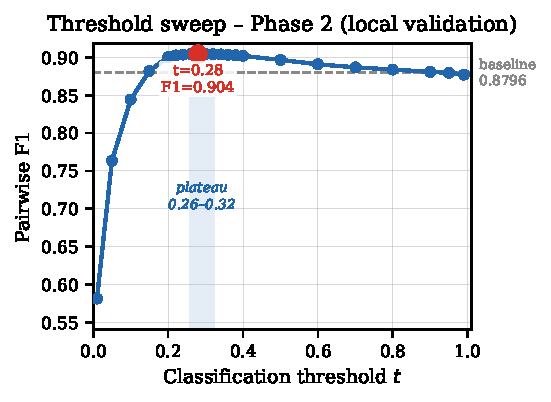
\includegraphics[width=\columnwidth]{fig_sweep.pdf}
  \caption{Pairwise F1 vs.\ classification threshold on local validation.
    The dashed line marks the cosine-similarity baseline (F1~=~0.8796).
    The shaded band shows the stable plateau; we submitted $t = 0.30$.}
  \label{fig:sweep}
\end{figure}

The F1 curve is flat between $t = 0.26$ and $t = 0.32$, indicating robust
performance in that range. We submitted $t = 0.30$ to the leaderboard
(leaderboard F1~=~0.9025) as the most conservative point in the plateau.

\textbf{Attempted extensions.}
Three extensions failed to improve over the baseline:

\emph{Anchor bridging.} Training items with known labels were used as
bridges: if two phase items both match the same training item at
$s \geq 0.92$, they are linked. In fashion, two distinct products can
both look similar to the same anchor (e.g., two different red dresses
resembling the same training dress), generating false bridges.
Leaderboard F1 dropped to 0.8866 (0.8888 with brand+dept filter).

\emph{Medium-similarity model.} A second XGBoost was trained on pairs
with $0.70 \leq s < 0.88$ to recover cross-geo pairs invisible to the
main model. The training positive rate was 25\%, but the inference
positive rate in this range is $\sim$0.1\% (a 250$\times$ class
imbalance), causing catastrophic over-merging (local F1~=~0.27).

\emph{Rule-based metadata promotion.} Pairs with brand + department +
colour exact match in the $0.70$--$0.88$ range were promoted. Brand
and department IDs are near-zero for most items in the dataset, so only
5 pairs qualified across the full inference set.

%% ── 6. Results ───────────────────────────────────────────────────────────────
\section{Results}

Our best submission achieves Pairwise~F1~=~\textbf{0.9025} on the Phase~2
leaderboard, compared to the cosine-threshold baseline of 0.8796 ($+0.023$).

\textbf{Error analysis.}
Inspecting the false-negative pairs reveals that the majority of missed
true matches have combined similarity $s < 0.70$ in the fine-tuned
embedding space. These are almost exclusively cross-geo pairs where (a)
titles are in completely different languages with no shared subword tokens
and (b) product photos have different backgrounds or cropping conventions.
The fine-tuned encoders reduce intra-language variance but do not fully
align cross-language representations. No post-processing step can recover
these pairs once they are absent from the FAISS candidate set.

\textbf{Ablation.}
The key ablation is the distribution mismatch experiment (Section~4).
A broadly-trained XGBoost with identical features and hyperparameters
completely fails (F1~$<$~0.10), whereas the distribution-matched model
achieves 0.9043. This 9-point absolute gap is the entire contribution
of the approach: not the features, not the encoder, but the alignment
between training and inference distributions.

%% ── 7. Conclusion ────────────────────────────────────────────────────────────
\section{Conclusion}

We presented a two-stage system for cross-geo product grouping: fine-tuned
multimodal encoders followed by a distribution-matched XGBoost pair
classifier. The central finding is that a reranker trained on the full pair
distribution is miscalibrated when applied to FAISS candidates, which form
a high-similarity subset. Restricting training to that exact region
(combined sim $\geq 0.88$) transforms a failing classifier into one with
AUC 0.9990 and achieves a leaderboard score of 0.9025.

The remaining performance gap (versus the top competitor at 0.9099) stems
from cross-geo pairs with $s < 0.70$, which are invisible to the FAISS
retrieval stage. Recovering these pairs would require stronger multilingual
alignment -- for example, training the text encoder with language-pair
supervision or using a cross-lingual alignment objective rather than purely
label-based contrastive loss. We leave this as the primary avenue for
improvement.

%% ── References ───────────────────────────────────────────────────────────────
\bibliographystyle{plain}
\begin{thebibliography}{9}

\bibitem{zalando}
Tóth, S., Wilson, S., Tsoukara, A., Moreu, E., Masalovich, A., Roemheld, L.
\textit{End-to-end multi-modal product matching in fashion e-commerce}.
arXiv:2403.11593, SIGKDD 2024.

\bibitem{glami}
Vanek, J. et al.
\textit{GLAMI-1M: A Multilingual Image-Text Fashion Dataset}.
FashionXRecsys Workshop, RecSys 2023.

\bibitem{ditto}
Li, Y. et al.
\textit{Deep Entity Matching with Pre-Trained Language Models}.
VLDB 2021.

\bibitem{deepmatcher}
Mudgal, S. et al.
\textit{Deep Learning for Entity Matching: A Design Space Exploration}.
SIGMOD 2018.

\bibitem{clip}
Radford, A. et al.
\textit{Learning Transferable Visual Models From Natural Language Supervision}.
ICML 2021.

\bibitem{faiss}
Johnson, J., Douze, M., Jégou, H.
\textit{Billion-scale similarity search with GPUs}.
IEEE Trans. Big Data, 2021.

\end{thebibliography}

\end{document}
